%!TEX root = ../thesis.tex
\chapter{Implementation}\label{implementation}

\ifpdf
    \graphicspath{{Chapter3/Figs/Raster/}{Chapter3/Figs/PDF/}{Chapter3/Figs/}}
\else
    \graphicspath{{Chapter3/Figs/Vector/}{Chapter3/Figs/}}
\fi

% \NOTE{D}{General note: This book https://d2l.ai/index.html has good references for the original papers.}


\section{\TwoThinning}



\NOTE{A}{\textbf{Precondition at this point: I expect the reader to understand Deep Q-Learning well enough, so that I just have to note some implementation details. The same should be true about \TwoThinning. If anyone who reads this dissertation finds the explanation so far insufficient, let me know.}}


\subsection{Deep Q-Learning Implementation} \label{dqn-implmentation-two-thinning}


As there is no prior work on RL for the discussed balls-into-bins setting, I implemented the RL algorithms from scratch using PyTorch for the NNs. Even though there are some attempts at general purpose RL libraries (e.g.\ Stable Baselines~\cite{hill2018stablebaselines}), they are very hard to customise at the moment. Following standard terminology, I will call the NN used by Deep Q-Learning as a Deep Q-Network (DQN).\NOTE{D}{Why not introduce this terminology in Chapter 2?} To discuss the implementation of Deep Q-Learning for \TwoThinning, I need the following definition.


There are two ways to formulate the \TwoThinning setting as a\NOTE{D}{an} MDP. One is to treat (load vector, primary bin) pairs as states, and accept/reject as actions. The other is to treat load vectors as states, and thresholds for accepting/rejecting as actions. I chose the latter, because it implicitly restricts the search space to be explored by the RL agent to slicing strategies, which is justified by the following important (also intuitive) lemma:


\begin{lemma} \label{lemma: thresholdproperty}
There exists a slicing strategy that achieves the optimal expected final maximum load.
\end{lemma}


Before proving this lemma, we need three more definitions and another lemma.


\begin{definition} [majorisation]
A vector $x$ is majorised by a vector $y$ (both of length $n$), denoted by $x \preccurlyeq y$ iff $$\sum_{i=0}^j x[i] \leq \sum_{i=0}^j y[i]\mathrm{, for\ all\ j\in [n]}$$. In other words, all the prefix sums of $x$ are smaller than the corresponding prefix sums of $y$.
\end{definition}


\begin{definition} [allocation probability vector]
For a sorted load vector $v$ and decision strategy $f$, we define the \textit{allocation probability vector} $P^f_v$: $P^f_v[i]$ is the probability of allocating the next ball at load vector $v$ into bin $i$ (the $i$th least loaded bin) according to $f$. For \TwoThinning, we can decompose $P^f_v$ into $P^f_{v1}+P^f_{v2}$, denoting the primary and secondary allocation probability vectors respectively.
\end{definition}


\begin{lemma} [simplified version of Theorem 7 of~\cite{azar1999twochoice}] \label{lemma: majorisation-implies-better}
If for two strategies $f$ and $g$, and every load vector $v$, $P^f_v\preccurlyeq P^g_v$, then $E^g\leq E^f$.
\end{lemma}

\begin{remark}
The proof in~\cite{azar1999twochoice} proceeds by applying a coupling between the two strategies and then showing by induction that the load vectors from $g$ are majorised by the load vectors from $f$ at each step.
\end{remark}


\begin{definition} [\TwoThinning inversions]
Let's call a load vector $v$ and indices $0\leq i<j<n$ an \textit{inversion} of a strategy $f$, if $f(v,i)=\mathrm{reject}$ but $f(v,j)=\mathrm{accept}$. Let's denote the number of inversions of a strategy by $I^f$, and the number of inversions for a fixed $v$ by $I^f_v$.
\end{definition}


\begin{proof} [Proof of Lemma~\ref{lemma: thresholdproperty}]
    The proof proceeds by contradiction. Assume there is no optimal slicing strategy, so take an optimal non-slicing decision strategy $f$ with the least number of inversions $I^f$. Since $f$ is non-slicing, $I^f\geq 1$, so take an arbitrary sorted load vector $v$ with $I^f_v\geq 1$. Let $a=\argmin_{i\in [n]} f(v,i)=\mathrm{reject}$ and $b=\argmax_{i\in [n]} f(v,i)=\mathrm{accept}$. Let $g$ be a new strategy defined by $g(v,a)=\mathrm{accept}$, $g(v,b)=\mathrm{reject}$ (``swapping'' the decisions of $f$) and otherwise acting exactly as $f$. Now I show that for all load vectors $w$, $P^f_w\preccurlyeq P^g_w$.
    
    When $w\neq v$, $P^f_w = P^g_w$ by construction, so $P^f_w\preccurlyeq P^g_w$. For $w=v$, note that $P^g_{v1}=P^f_{v1}+\frac{1}{n}\cdot e_a-\frac{1}{n}\cdot e_b$, where $e_i$ denotes the $i$th basis vector. We have $P^f_{v1}\preccurlyeq P^g_{v1}$, because for $0\leq i<a$ and $b\leq i<n$, $\sum_{j=0}^i P^f_{v1}[j] = \sum_{j=0}^i P^g_{v1}[j]$, and for $a\leq i<n$, $\sum_{j=0}^i P^f_{v1}[j] + \frac{1}{n} = \sum_{j=0}^i P^g_{v1}[j]$ (intuitively, a probability of $\frac{1}{n}$ has been moved to the left). Now observe that $P^f_{v2}=P^g_{v2}$, because the number of rejects among $f(v,i)$ ($i\in [n]$) overall are the same as the number of rejects among $g(v,i)$ ($i\in [n]$) overall. Hence, because $P^f_{v1}\preccurlyeq P^g_{v1}$, and adding a constant $P^f_{v2}=P^g_{v2}$ doesn't change majorisation, we get $P^f_v \preccurlyeq P^g_v$.
    
    
    Since $P^f_w\preccurlyeq P^g_w$ for any load vector $w$, Lemma~\ref{lemma: majorisation-implies-better} implies $E^g\leq E^f$. $I^g<I^f$, because for $w\neq v$, $I^g_w=I^f_w$, and for $w=v$, the ``swap'' removed (at least) the inversion $(v,a,b)$, and didn't introduce any new inversions (see Figure~\ref{two-thinning-swap-action}). Hence, either $E^g<E^f$, or $E^g=E^f$ but $I^g<I^f$, contradicting the original assumption.
\end{proof}


\begin{remark}
Lemma~\ref{lemma: thresholdproperty} has also been verified by the \DP strategy (defined later in Section~\ref{two-thinning-dp}) for small values of $n$ and $m$.
\end{remark}



\begin{figure}
    \centering
    %\includegraphics{} TODO
    \caption{The ``swap'' action for \TwoThinning}
    \label{two-thinning-swap-action}
\end{figure}


\subsubsection{Deep Q-Network (DQN)} \label{DQN}

The input to the DQN is a representation of the load vector $v$, and the output is an estimate of $Q(v, a)$ for each possible threshold $a$. We can observe the following constraints on the possible values of $a$:

\begin{itemize}
    \item It is enough to consider only\NOTE{D}{remove only} integer thresholds, as the load values are integer too\NOTE{D}{as the loads are integers}.
    \item It is always optimal to accept a bin with load $0$ (this is a corollary\NOTE{T}{It is, but maybe a bit more detail need to be added.} of\NOTE{D}{Replace with ``see Lemma ??''} Lemma~\ref{lemma: thresholdproperty}), so $a\geq 0$.
    \item Thresholds $a$ larger than the maximum possible load $m$ have the same effect as using $a=m$.
    \item It is well-known that \OneChoice -- a less powerful protocol than \TwoThinning -- has a final maximum load less than\NOTE{T}{the use of ``less than'' is quite confusing... I think you rather want the lower bound here, but if you write $\Theta$ it is indeed a lower and upper bound.} $\Theta (\frac{m}{n} + \sqrt{\frac{m\log n}{n}})$\NOTE{D}{$m/n + \Theta(\sqrt{\frac{m\log n}{n}})$} with high probability~\cite{raab1998onechoice}. Therefore, we can further limit the search space by allowing only thresholds less than a chosen \textit{max threshold}. For the exact value of this hyperparameter and all the other hyperparameters explained later in this chapter (e.g.\ learning rate, hidden size of NN layers), see Appendix~\ref{hyperparameters}. \NOTE{A}{This is important! If they miss it, I expect to lose around 20 marks. Any better place to put it but avoid the out of nowhere effect?} \NOTE{D}{Maybe mention it once more in Chapter 4.}
    
\end{itemize}


Now, I will explain the input representation for the DQN.\NOTE{D}{Maybe just change to ``paragraph{Input representation}''?} First of all, I always sort the load vector before feeding it into the network. This is possible because the order of the bins does not matter in \TwoThinning, unlike in \GraphicalTwoChoice. Sorting improves learning as the NN does not have to learn permutation invariance~\cite{zaheer2017permutationinvariance}, and it will be important\NOTE{D}{Do you show this in the evaluation?} also for the actual NN architecture I use. Then, I one-hot encode each load value independently, because NNs often cannot learn well with ordinal data. I use the natural $0$-$m$ range for one-hot encoding, but to reduce the number of weights of the NN I tried collapsing the very high load values (that have very small probability of occurring), into one ``outlier'' class, as shown in Figure~\ref{NN-maxload}. This didn't provide better results\NOTE{D}{Did it provide the same results? It must have reduced the number of parameters.}, so I do not discuss it any further.

\NOTE{D}{This paragraph can be made a bit more concise: ``I sorted the load vectors and represented them using a one-hot encoding in the range $[0, m]$. Sorting improves ... . One-hot encoding is motivated since NNs cannot learn well with ... . I also tried compressing the largest values, ... }

\begin{figure}[h]
    \centering
    %\includesvg[scale=0.15]{Chapter2/Figs/NN_maxload.svg} -- it completely messes up the dots on the image
    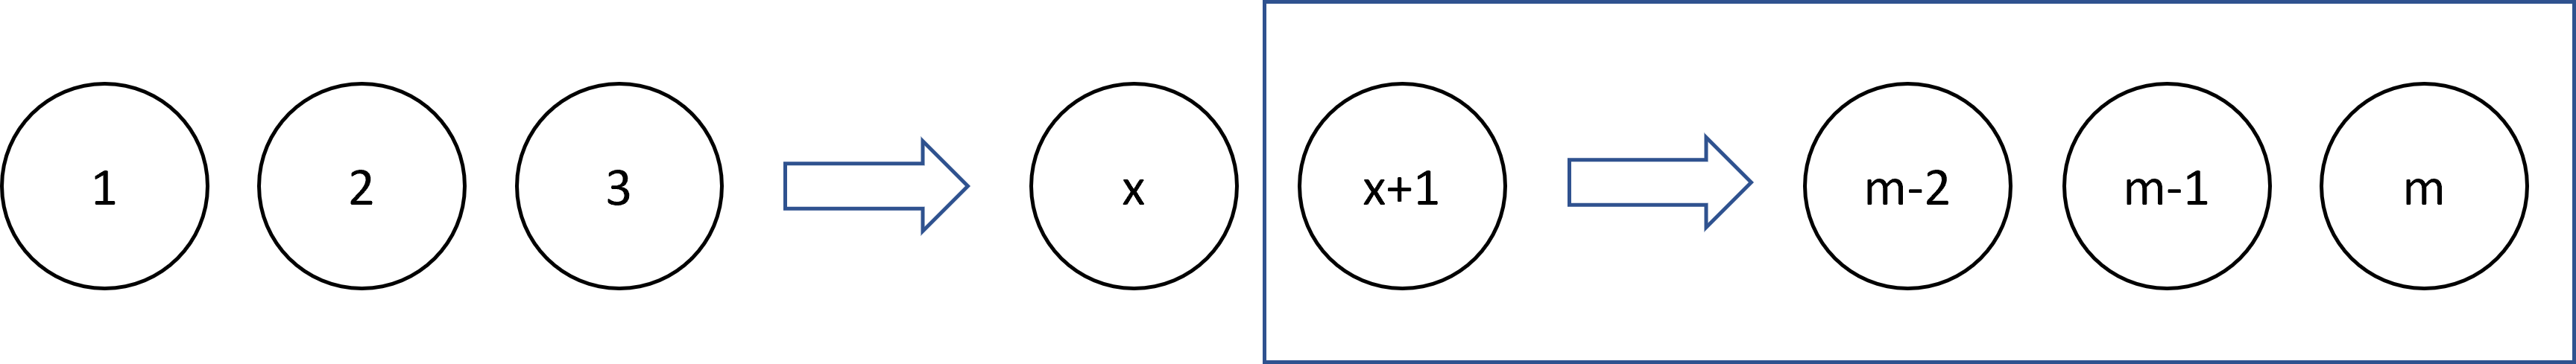
\includegraphics[scale=0.5]{Chapter2/Figs/NN_maxload.png}
    \caption{Potential grouping of (increasing) load values for one-hot encoding.}
    \label{NN-maxload}
\end{figure}
\NOTE{D}{``Potential'' to ``A possible grouping of'}
\NOTE{T}{I think having a figure here is a good idea, but I'm no sure the figure is a good illustration...}

Now I turn to the discussion of the actual architecture of the DQN.\NOTE{D}{Maybe ``paragraph{DQN architecture}''} Arguably, the highest loaded bins of a load vector are more important bins, since we care about minimising the maximum load.\NOTE{D}{Would be nice if you could support this in the evaluation. Andor: agree, it would be nice. Any specific ideas? Sounds difficult to analyse.}\NOTE{D}{You could flip the load vector and show that the results are worse.}\NOTE{T}{To me this claim is a bit ``bold''. If you want to balance well in the long-term, you may really have to look at all load values and not just the two or three highest.} In the extreme, if the bin with the maximum load contained one more ball, that would be more significant than if an average loaded bin contained one more ball. Hence, my idea was to process the load vector in increasing order of the (one-hot encoded) loads, that is, in increasing order of importance. For this purpose, using a vanilla RNN -- which processes sequential data, inherently focusing more on later inputs -- is a perfect choice.\NOTE{D}{This sentence does not justify why ``vanilla RNN is the perfect choice''. You could just say that you used an RNN to encode the load sequence.} I also tried the two more complex versions of RNNs (GRU, LSTM) mentioned in Section~\ref{RNN}, but even though their\NOTE{D}{they have} desirable properties, they could not provide any improvement (partly due to the fixed-sized, relatively short\NOTE{D}{These are not short sequences} input sequences \NOTE{A}{Should I be more confident or say that "probably" or "I hypothesise"?}), so I do not discuss them any further. \NOTE{D}{Would be good to refer to a figure in the evaluation section. Andor: yes, but there is no space to evaluate and compare exactly everything. Isn't it valid if I decide not to discuss it any further and focus on other things in the evaluation?}\NOTE{D}{OK, though it is quite common to have an ablation study.}.
The hidden state of the RNN after the last input is fed through some number of fully connected (linear)\NOTE{D}{Remove linear?} layers to produce the estimates for $Q(v, a)$. As for the activation functions, I use ReLU for the linear layers, and $\tanh$ activation inside the RNN, following common practice (see e.g.~\cite{szandala2020activationfunctions}).


\subsubsection{Stabilising Training}


In practice, Deep Q-Learning\NOTE{D}{See my comment for replacing all these with DQL} -- and in general any off-policy deep reinforcement learning algorithm -- can become unstable during training. There are several methods proposed in the literature to address this issue, and I implemented three of them that work well together in practice (see e.g.~\cite{mnih2015dqnstabilitycombined}).


\paragraph{Experience Replay}
\NOTE{D}{Maybe start by what happens in your setting when you apply the vanilla Deep Q-Learning algorithm. And then mention how ``experience replay~~\cite{lin1992experiencereplay}'' solves this problem. }
\NOTE{D}{It might be helpful to split the paragraph into two: (i) what is experience delay and the problem it solves, (ii) how you implemented it}

Experience replay~\cite{lin1992experiencereplay} is trying to solve\NOTE{D}{aims to address} the problem that in vanilla Deep Q-Learning, subsequent update steps are correlated -- e.g.\  in our case, after we update the weights of the DQN around a load vector with $x$ balls, we next update it around a load vector with $x+1$ balls. This correlation stems from updating in the same order as executing the actions in the game. In order to get the theoretical guarantees for these supervised learning-like updates, we need to have independent i.i.d. training samples. The idea in experience replay, is that instead of calling the update rule~\ref{eq:deep-q-learning-update-with-semi-gradient} on the current $(s, a, s', r)$ tuple, we store this tuple in an experience replay buffer. Then, after every fixed number of steps, a batch of tuples are sampled uniformly at random from the buffer, and the DQN is updated according to those tuples. Another benefit of the idea is that samples can be reused multiple times, leading to a more efficient learning. Nevertheless, there should be a size limit on the buffer to get rid of outdated samples, which I implemented using a deque data structure with a limited memory capacity. Finally, note that sampling a batch of tuples rather than a single sample when updating has been shown to have a stabilising effect~\cite{qian2020batchingsgd}.


\paragraph{Target Network}


The main difference between Q-Learning and Deep Q-Learning is that in the former, during one step we only update a single value in the Q-table, while in the latter, due to the function approximation, many neighbouring values are also affected. This becomes problematic, since looking at the update rule~\ref{eq:deep-q-learning-update-with-semi-gradient} for Deep Q-Learning, to update around a Q-value $Q_{\mathbf{w_t}}(s_t, a_t)$, a neighbouring Q-value $Q_{\mathbf{w_t}}(s_{t+1}, a')$ is used. This can lead to a blow-up in the Q-values, intuitively, as a chain reaction. The idea with target networks\NOTE{D}{Just ``Target networks have two copies''?}~\cite{argueta1992targetnetwork} is to have two copies of the same network architecture: one whose weights are updated by the update rule, and one that provides $Q_{\mathbf{w_t}}(s_{t+1}, a')$ of the ``target'' part $r_{t+1}+ \max_{a'} Q_{\mathbf{w'_t}}(s_{t+1}, a')$ of the rule. This weights $w'$ of the target network are updated to that of the main network periodically, every fixed number of training episodes. Another way to think about this is \NOTE{D}{as} a way to achieve the stability of~\ref{eq:deep-q-learning-update-with-semi-gradient}, while still using the full gradient descent update rule.


\paragraph{Using a better Optimiser}


Expanding on \NOTE{D}{the}update rule~\ref{eq:deep-q-learning-update-with-semi-gradient}\NOTE{D}{\eqref{eq:deep-q-learning-update-with-semi-gradient}}, which updates the weights (based on the gradient) using simple Stochastic Gradient Descent (SGD), SGD could be replaced by any other (more complex) optimiser, such as ADAM~\cite{kingma2015adamoptimiser}. Briefly, it additionally adjusts the step size based on moving averages and variances of the gradient. I also added gradient clipping \cite{mikolov2012gradientclippingoriginal}, a widely used extension in deep reinforcement learning, which does not allow absolute gradient values to exceed $1$, hence prevents exploding gradients and has been shown to also speed up training~\cite{zhang2020gradientclippingaccelerate}.



\subsection{Ideas Implemented for Improvement} \label{improvementideas}


In this section I outline ideas independent of the DQN that I implemented to improve the performance of my RL algorithm. Some of these are well-known general ideas in RL, while others are specific to the \TwoThinning balls-into-bins setting.


\subsubsection{Reward Shaping} \label{rewardshaping}

As discussed in Section~\ref{RLintro}, the most direct way to formulate the \TwoThinning setting as a MDP is to only give a reward (equal to minus the maximum load) after a final state, i.e.\ when all the balls have been allocated. The problem with this is that rewards are very sparse -- concretely, the agent only receives one reward per episode. It\NOTE{D}{This} is problematic because until the final rewards propagate back to earlier states (that is, load vectors with fewer balls), the updates at earlier states are not justified -- they use a zero reward and a randomly initialised next state to update the current state. Hence, the idea is to inject\NOTE{D}{Reward shaping injects} additional rewards into the MDP, while \NOTE{D}{The rest of the sentence is a bit hard to read. Maybe ``while still converging to the original optimum?}maintaining correctness: the optimal policy for the new modified MDP has to be optimal for the original one as well, and hence for the \TwoThinning protocol too. There is a very interesting result proved in~\cite{ng1999rewardshaping} about exactly what extra rewards can be used while maintaining the same optimal and near-optimal policies: the extra reward, when moving from state $s$ to state $s'$ using action $a$ has to be in the form $\Phi(s')-\Phi(s)$, i.e.\ the difference of the so-called potential functions $\Phi$ of the two states. Intuitively, the potential function should denote an estimate of how good a state is with respect to the original (in our case final) rewards. Now I present the candidate\NOTE{D}{remove candidate?} potential functions that I have created:

\begin{itemize}
    \item
    $\Phi_{max}(v)=\mathrm{maxload}(v)=- \max_{i \in [n]} v[i]$\NOTE{D}{Sometimes you use $v[i]$ and others $v_i$}, which naturally extends the final reward. This means that the reward is $-1$ if the ball is allocated to a bin with maximum load, otherwise $0$.
    \item
    $\Phi_{std}(v)=-\mathrm{std}(v)$, where $std(v)$\NOTE{D}{$\mathrm{std}$} is the standard deviation of the load vector. Compared to $\Phi_{max}$, it differentiates also between bins with non-maximum load.
    \item
    $\Phi_{exp}(v)=\sum_{i \in [n]} e^{\alpha \cdot  (v[i] - \mathrm{avg}(v))}$, with $\alpha>0$ a hyperparameter controlling the steepness of the function as shown for an individual load value in Figure~\ref{exponential-potential-alpha}, is the so-called\NOTE{D}{Remove so-called} exponential potential\NOTE{D}{italics}, which has first been \NOTE{D}{used for theoretical analysis of balls-into-bins processes. (Maybe mention in the introduction that it has not been used to guide the choice of a protocol?)}introduced as a useful tool in proving bounds for balls-into-bins settings~\cite{ghosh1999exponentialpotential}. As a relevant example\NOTE{D}{Replace with ``Note taht when''?},\NOTE{D}{Mention that this is a smoother version of the first one. Andor: what do you mean? I don't get it.}\NOTE{D}{I meant that as $\alpha \to \infty$, only the term corresponding to the maximum load matters.} if the exponential potential of a load vector $v$ is $O(n)$, it follows that $\mathrm{maxload}(v) < \mathrm{avg}(v)+O(\log(n))$.
\end{itemize}


\begin{figure}[h]
    \centering
    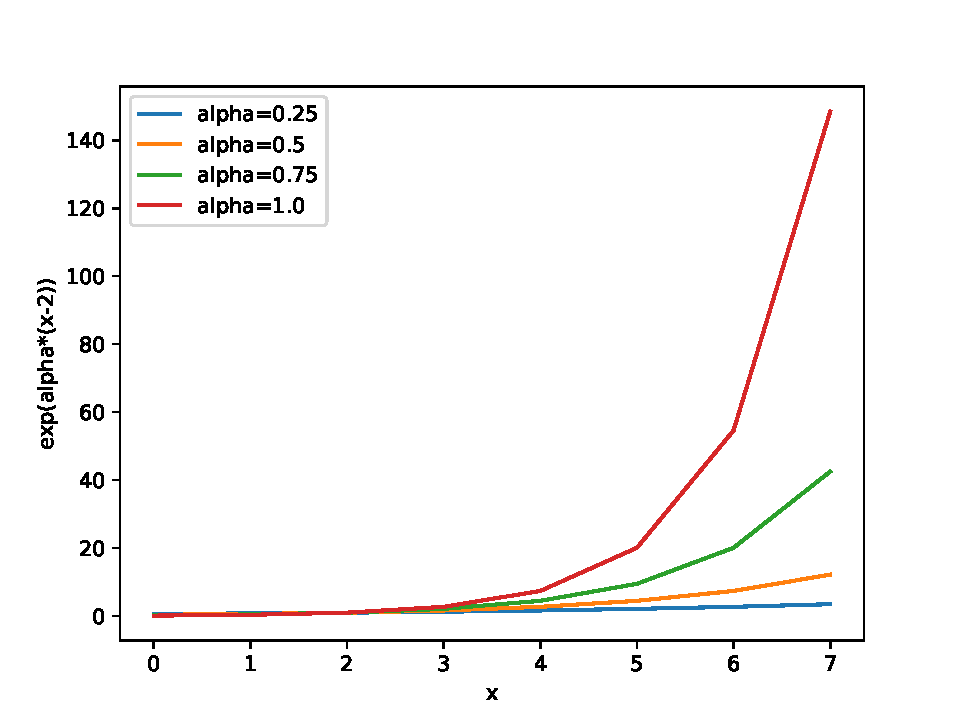
\includegraphics[scale=0.7]{Chapter3/Figs/exponential_potential_analysis.pdf}
    \caption{Showing the effect of different values of $\alpha$ to the exponential potential function with an average load of $2$.}
    \label{exponential-potential-alpha}
\end{figure}



\subsubsection{Curriculum Learning}


The idea of curriculum learning\NOTE{D}{Maybe ``Curriculum learning first provides easier ...'' }~\cite{bengio2009curriculumoriginal} is to first provide easier problems to the agent, and just gradually increase the difficulty up to the original problem. I used this method as a pretraining phase for some number of \textit{pretrain episodes}. Without curriculum learning, the agent cannot learn as much as desired from the hard problems initially \NOTE{A}{Explain some more?}\NOTE{D}{it would be nice to have some empirical evidence to support this in the evaluation section.}. For \TwoThinning, I implemented curriculum learning by first providing\NOTE{D}{I first provided laod vectors with ..., then with .. } load vectors with $m-1$ balls allocated, then providing load vectors with $m-2$ balls allocated, and so on until starting from the original empty bins. To choose the training samples on level $k$ (i.e.\ where to place the initial balls), I had to choose load vectors with $m-k$ balls that are ``relevant'' -- there are exponentially many ways to place $m-k$ balls into $n$ bins, so it is not feasible to provide each of them to the agent. The heuristic I chose was to run the vanilla \OneChoice protocol with $m'=m-k$ balls, providing training samples distributed according to their occurrence when running \OneChoice, which is a closely related protocol to \TwoThinning. I decided to distribute the iterations between the levels according to an arithmetic progression, putting more weight on smaller $k$'s.
\NOTE{D}{This is quite interesting, but the description could be slightly improved.}



\subsubsection{Normalised Domain} \label{normalised-domain}

The notion of normalised loads\NOTE{D}{Maybe: ``Normalising loads proved to be ''?} mentioned in Section \ref{assumptions} proved to be a very useful trick\NOTE{D}{remove trick?} for RL training as well. Extending the notion to normalised thresholds (a normalised threshold $c$ at timestep $t$ is equivalent to a threshold $c+\frac{t}{n}$), we can consider slicing strategies with a constant \textit{normalised} threshold $c$. Unlike for constant \textit{unnormalised} thresholds, $c=0$ already gives a reasonable strategy (``\MeanThinning'')~\cite{los2022cachingpackingthinningtwinning}, and learning a constant output is easy for a NN already in the early episodes.


\subsection{Dynamic Programming} \label{two-thinning-dp}


For smaller values of $n$ and $m$ we can use dynamic programming (DP) based on the Bellman equation~\ref{eq:bellmanState} to get the exact optimal policy (``\DP strategy'') and its expected final maximum load. Now I present some observations that allow dynamic programming for a larger set of $n$ and $m$:


\begin{itemize}
    \item 
    Like for\NOTE{D}{As in?} the DQN, we can reduce the state space by $\Theta(n!)$, due to permutation invariance.
    \item
    In the MDP formulation of \TwoThinning, there is no cycle in the state transition graph, because the number of balls is always increasing. Therefore, instead of performing a fixed point iteration~\cite{rhoades1991fixedpointiteration}, we can directly calculate the state values based on recurrence relation \ref{eq:twothinning-dynamicprogramming}.
    \item
    Exploiting Lemma~\ref{lemma: thresholdproperty}, I use sorted load vectors as states, and not (sorted load vector, threshold) pairs. I also implemented a slower version without using Lemma~\ref{lemma: thresholdproperty}, to verify the correctness of the Lemma, and of the implementation of the faster algorithm.\NOTE{D}{I think you should describe these a bit more.}
\end{itemize}


Denoting $v[i]$ as the $i$th smallest load value in the load vector $v$\NOTE{D}{This should be in Chapter 2. You have already used this before.}, and $e_j$ as the corresponding unit vector $(0, 0, ... , 1, ..., 0, 0)$: \NOTE{T}{What is the range of $i$? Is it $i=1,2,\ldots,n$? But then you need to update the formula below. Andor: it is from $0$ to $n-1$. Why do I need to update anything?}
\NOTE{D}{Mention that this is for $v$ with $\sum_{i = 1}^n v_i < m$}
\begin{equation} \label{eq:twothinning-dynamicprogramming}
\begin{split}
    V_{\pi^*}(v) &= \max_a \mathbb{E} [r_t + V_{\pi^*}(s_{t+1}) \mid s_t=v, a_t=a] \\
    &= \max_{i \in [n]} \mathbb{E} [r_t + V_{\pi^*}(s_{t+1}) \mid s_t=v, a_t=v[i]] \\
    &= \max_{i \in [n]} \left(\sum_{0\leq j \leq i} \frac{1}{n}\cdot V_{\pi^*}(v+e_j) + \frac{n-i-1}{n} \cdot  \sum_{j \in [n]} \frac{1}{n}\cdot V_{\pi^*}(v+e_j) \right)
\end{split}
\end{equation}
where we used the fact that $r_{t+1}=0$ for non-final states, and that it suffices to use only thresholds that are equal to one of the load values.\NOTE{D}{Give references to the Lemmas proving these properties.} The base cases are load vectors $v$ with $m$ balls allocated, and for those we have $V_{\pi^*}(v)=-\mathrm{maxload}(v)$. Since the base cases are difficult to enumerate in this problem, I implemented the algorithm using recursion and memoisation. 


We can observe that having already calculated $(\sum_{0\leq j \leq i} \frac{1}{n}\cdot V_{\pi^*}(v+e_j) + \frac{n-i-1}{n} \cdot  \sum_{j \in [n]} \frac{1}{n}\cdot V_{\pi^*}(v+e_j))$ for $i$, calculating it for $i+1$ takes $O(1)$ time, since only a constant number of terms change, and the $\sum_{j \in [n]} \frac{1}{n}\cdot V_{\pi^*}(v+e_j)$ term can be pre-calculated before looping through the possible thresholds. This gives an extra $\Theta(n)$ speeding, giving $\Theta(|states|\cdot n)$ as the overall time complexity of the algorithm. The space complexity is $\Theta(|states|)$.\\


Now I prove a small lemma limiting the possible improvements of any exact dynamic programming algorithm:\NOTE{T}{Why is this lemma limiting the improvements of DP? I think the lemma is ``only'' saying that with some small probability, you can get an arbitrarily bad load configuration.}


\begin{lemma} \label{lemma: everystatereachable}
For any load vector $v$ with $0\leq x\leq m$ balls in it\NOTE{T}{in it does not sound very nice. Why not just ``For any load vector with $m$ balls,''?}, and any strategy, there is a non-zero probability of reaching $v$ during an execution.
\end{lemma}

\begin{proof}
    Simply observe that if the primary and secondary bins are the same, then whatever strategy is used, the ball will be allocated in that bin, so any ball can go to any bin with a non-zero probability.
\end{proof}
\NOTE{A}{A more interesting question is what would happen if we disallow the two choices to be the same. Then, there are several load vectors that the optimal policy can avoid, e.g.\ (0,0,0,0,m,0,0). How can we characterise these vectors?}
\NOTE{T}{I'm not sure you could reduce the space by that much. I think you can probably still get load vectors like (m/2,m/2,0,...,0).}

This means that all the possible states have to be taken into account when calculating the expected maximum load.



Interestingly, there is no closed-form formula for the number of states. \NOTE{T}{Maybe cut this paragraph from here, or completely?} Even for $m=n$, when the number of states equal the so-called partition function $p(n)$, only approximate results are known: $p(n) \sim e^{\sqrt{n}}$~\cite{hardy1918partitionfunction}. I implemented the calculation of the exact number of states $f(m, n)$ as a function of $m$ and $n$, i.e.\ the number of non-decreasing partitions of $m$ of size $n$, for which I also used dynamic programming:

\begin{equation} \label{eq: numberofpartitions}
    f(m, n) = \begin{cases}
        1, & \text{for } m=0,\\
        1, & \text{for } n=1,\\
        f(m,n-1)+f(m-n,n), & \text{otherwise}.
    \end{cases}
\end{equation}




The values of $f$ confirmed the empirical performance of the DP algorithm.

\iffalse % I think it is enough if I mention this just in the evaluation
For example, for $n=10$, $m$ cannot exceed $60$, and for $n=30$, $m$ cannot exceed around $45$ so that it runs in time comparable to the training of Deep Q-Learning (few hours).\NOTE{D}{You will need to add a figure in the evaluation section.} These limits are indeed smaller than that of Deep Q-Learning, so while dynamic programming can provide the exactly optimal policy, it is not applicable for larger values. I note that the difference in the range of applicability of the two algorithms is perhaps surprisingly not very large\NOTE{D}{Are you sure?}. The main drawback of the dynamic programming algorithm is rather that it does not use function approximation, so it has to represent every state explicitly, which would cause memory error even before it would take too much time. \NOTE{A}{Add these rough estimates of n,m to Deep Q-Learning as well.}
\fi

\subsection{Other Strategies}

In addition to the strategies given by RL and DP, I implemented several other, more ``manual'' strategies. I provide a thorough comparison in Chapter~\ref{evaluation}.


\paragraph{\AlwaysAccept strategy}
This is equivalent to \OneChoice, and it is included as a baseline. This is very robust, and requires no centralised information in a practical implementation.


\paragraph{\MeanThinning strategy}
This strategy always accepts a ball if it is below the current average load, and rejects otherwise. In a practical implementation, the only centralised element required would be a counter, and it has been shown that the performance does not decrease significantly if the counter is not exact~\cite{los2022cachingpackingthinningtwinning}. 


\paragraph{\LocalRewardOptimiser strategy}

While the goal of the RL agent is the\NOTE{D}{to} optimise the expected cumulative reward, a simplified goal can be optimising the expected immediate reward, For this strategy, I chose the $\Phi_{max}$ potential from Section~\ref{rewardshaping} for reward shaping, which leads to accepting any bin that does not have maximum load.\NOTE{D}{Maybe a short lemma saying that this is equivalent to avoiding the maximum?}


\paragraph{\Threshold strategy \protect\footnotemark[1]} 


\footnotetext[1]{The name of this strategy is from the original paper, but the word ``threshold'' is overloaded in this field.}

This is a strategy that has been shown to be optimal~\cite{feldheim2021thinning} up to a constant factor for large $n$, and $m = O(n \cdot \sqrt{\log n})$. This strategy accepts a bin, if and only if the number of \textit{primary allocations} (i.e.\ number of times that bin has been chosen as the primary bin and it has been accepted by the strategy) to that bin so far are less than a constant $l$, which is set to $\sqrt{\frac{2\log n}{\log \log n}}$ in~\cite{feldheim2021thinning}. Note that this is not a slicing strategy, as the decisions are not even based on the actual load values. To the best of our knowledge, the reason for this reliance on the primary allocations instead, is to aid the proofs in the paper, and it also leads to an easily expressible strategy. The strategy performs worse if $m$ is much larger than $n$, because $l$ is constant and the strategy is not ``adaptive''. It can be implemented without any shared state, by each bin keeping track of its own primary allocations.

\section{\KThinning}


\subsection{Deep Q-Learning Implementation}


To formulate the \KThinning problem as a MDP, I decided to use (load vector, number of choices left) pairs as states, and just like for \TwoThinning, thresholds as actions. The ``number of choices left'' part of the states indicate how many more bins can be rejected before the ball would be allocated into a randomly chosen bin. The state transitions happen according to the definition of \KThinning. To tackle the sparse reward problem, I decided to use the same potential functions as for \TwoThinning (hence not taking into account the number of choices left) to avoid introducing unnecessary bias for the agent.


For the DQN, I extended the architecture for \TwoThinning by concatenating the final hidden state of the RNN with the one-hot encoded representation of the number of choices left, feeding them together to the linear layers. The rest of the implementation is analogous to \TwoThinning.



\subsection{Dynamic Programming}


\NOTE{D}{I implemented ..}A DP algorithm analogous to that for \TwoThinning has been implemented for \KThinning as well, with the states being (sorted load vector, number of choices left) pairs.


The recurrence equations are:
\begin{align} 
    V_{\pi^*}((v, 0)) &= \max_a \mathbb{E} [r_{t+1} + V_{\pi^*}(s_{t+1}) \mid s_t=(v,0), a_t=a] \notag \\
    &= \max_{i \in [n]} \mathbb{E} [r_{t+1} + V_{\pi^*}(s_{t+1}) \mid s_t=(v,0), a_t=v[i]] \notag \\
    &= \max_{i \in [n]} \left(\sum_{0\leq j \leq i} \frac{1}{n}\cdot V_{\pi^*}((v+e_j,k)) + \frac{n-i-1}{n} \cdot  \sum_{j \in [n]} \frac{1}{n}\cdot V_{\pi^*}((v+e_j,k))\right), \label{eq:kthinning-dynamicprogramming} \\
    V_{\pi^*}((v, x+1)) &= \max_a \mathbb{E} [r_{t+1} + V_{\pi^*}(s_{t+1}) \mid s_t=(v,x+1), a_t=a] \notag \\
    &= \max_{i \in [n]} \mathbb{E} [r_{t+1} + V_{\pi^*}(s_{t+1}) \mid s_t=(v, x+1), a_t=v[i]] \notag \\
    &= \max_{i \in [n]} \left(\sum_{0\leq j \leq i} \frac{1}{n}\cdot V_{\pi^*}((v+e_j,k)) + \frac{n-i-1}{n} \cdot  V_{\pi^*}((v, x))\right).
\end{align}

\NOTE{A}{How to make the two aligned? I would love to group them somehow but couldn't find anything.}

The runtime of this algorithm is $k$ times the runtime of the DP algorithm for \TwoThinning: $\Theta(|states|\cdot n\cdot k)$.\NOTE{D}{You have a symbol $S$ for states?}


\subsection{Other Strategies}

Similar kinds of strategies are possible for \KThinning as for \TwoThinning, with some adjustments.

\paragraph{\AlwaysAccept strategy} Same as for \TwoThinning.


\paragraph{\Quantile strategy} This strategy accepts a ball if there is less than $0.5$ probability of getting a better offer at later choices. To find this corresponding quantile $y$ with $x$ choices left, we solve the following equation:

\begin{equation} \label{quantilekthinning}
1 - (\frac{n-y}{n})^x = \frac{1}{2}
\end{equation}

which gives $y = n \cdot  (1 - 2^{-\frac{1}{x}})$, and then the threshold is $v[\floor{y}]$ where $v$ is the sorted load vector. \NOTE{A}{Explain better?}. Note that we could instead extend the \MeanThinning Strategy from \TwoThinning directly, but I do not consider that any further as that does not adapt to $k$.


\paragraph{\LocalRewardOptimiser strategy} Choosing according to the expected immediate reward based on the $\Phi_{max}$ leads to rejecting any bin with maximum load, and accepting otherwise.


\paragraph{\Threshold strategy} This is a direct of extension of the analogous strategy for \TwoThinning: it accepts the $i$th choice if the number of times a ball has been allocated to that bin as the $i$th choice so far is not greater than a constant $l$. This strategy\NOTE{D}{Maybe say an instance of this?} has been shown to be asymptotically optimal~\cite{feldheim2020dthinning}.


\section{\GraphicalTwoChoice}


\subsection{Deep Q-Learning Implementation} \label{graphical-DQN}

Since Lemma \ref{lemma: thresholdproperty} cannot be extended to \GraphicalTwoChoice, to formulate the MDP I simply take (load vector, (bin1, bin2)) tuples as states, and the boolean choice between the two bins as actions. On the other hand, for the DQN, to avoid index-valued input, I use the load vector as the input, and the Q-value estimates for each bin as the output. Then, I choose between bin1 and bin2 by comparing the two estimates. Note that sorting the load vector would in this setting would ignore the graph structure. Hence, without any sensible order for the bins, I decided to replace the RNN (used for sequential processing) by a fully connected network which can possibly make use of the connectivity information. As future work, Graph Neural Networks (GNN) \cite{scarselli2009GNN} could be tried as well,\NOTE{D}{Remove the rest of the sentence?} but their application to this problem is not straightforward.



To tackle the sparse rewards problem, I propose graph-aware potential functions. The motivation is that for example two heavily load bins can lead to much higher maximum load if they are connected, or even close to each other in the graph, than if they are distant.


\begin{itemize}
    \item 
    $\Phi_{edge}(v)=\max_{x\sim y \in E} \min(v[x], v[y])$, finding the ``worst'' edge in the graph.
    \item
    $\Phi_{neigh}(v)=\max_{x \in [n]} \frac{v[x]+\sum_{x\sim y \in E}v[y]}{\deg(x)+1}$, i.e.\ finding the neighbourhood with the largest average.
\end{itemize}


\subsection{Dynamic Programming}

Using load vectors as states, denoting the graph by $G$, its edges by $E$, and assuming that the nodes are numbered from $0$ to $n-1$\NOTE{D}{You are already making this assumption because the nodes are just the bins.}, I use the following recurrence relation for general graphs:


\begin{equation} \label{eq:graphicaltwochoice-dynamicprogramming}
    V_{\pi^*}(v) = \frac{\sum_{x\sim y}\max_a (V_{\pi^*}(v+e_x), V_{\pi^*}(v+e_y))}{|E|}
\end{equation}
and we have\NOTE{D}{and using that} $V_{\pi^*}(v)=-\mathrm{maxload}(v)$ for final states $v$.

This achieves an $\Theta(|states|\cdot |E|)$ algorithm, where $|states| = \sum_{x=0}^{x<m} {{x+(n-1)} \choose {x}} = {{m+(n-1)} \choose {m-1}}$, \NOTE{D}{$\sum_{x = 0}^{m-1}$}exponentially more than for \TwoThinning because equal loads are not interchangeable.

I will use this algorithm to construct a counterexample \NOTE{D}{where}that the \Greedy strategy (outlined below) is suboptimal.\NOTE{D}{Add reference to the lemma} For that purpose, I will distinguish not two, but three possible decisions: choose the first bin, choose the second bin, or both have the same expected value (neither is better than the other). The optimal decisions are easily derivable from the memoisation dictionary.


\subsection{Other Strategies} \label{graphical-otherstrategies}


\paragraph{\Greedy strategy} Choose the bin with the smaller load, or choose uniformly at random if they have the same load.


\paragraph{\Random strategy} Choose uniformly at random between the two bins. This is in bijection with \OneChoice.


\paragraph{\LocalRewardOptimiser strategy} In this case, the $\Phi_{max}$ potential function leads to choosing the ball which does not have maximum load, and choosing uniformly at random if they both or neither have maximum load.


\paragraph{Flow Based strategy}

\NOTE{D}{This is a very long description for something that was not implemented. Maybe just a sentence that there are other protocols, is ok?}The idea of the algorithm presented in~\cite{bansal2021twochoicegraphical} is to adjust the \Greedy strategy by comparing not simply the loads of the two offered bins, but the average loads in carefully chosen pre-computed neighbourhoods of size $O(\log(n))$ around the two bins, taking into account topological information as well (note that my potential function $\Phi_{neigh}$ is inspired by this algorithm). To define the aforementioned neighbourhoods, the algorithm represents the preferences as a particular multi-commodity flow problem, and solves it using an advanced data structure called a R\"{a}cke-tree~\cite{racke2008racketree}. I did not implement this algorithm due to its complexity (it could be a major part of a Part II project on its own)\NOTE{T}{Important: drop this bracket}, but I added it here as the best-known theoretical results for the \GraphicalTwoChoice setting, since it has been shown to be optimal up to a polylogarithmic factor~\cite{bansal2021twochoicegraphical}.



\subsection{Graph Structures}


Now I list the types of graphs on which I will evaluate the decision strategies. It is important that I train a separate RL agent for each graph, just like for each $n$, $m$ pair.


\paragraph{Complete graph} This is exactly the \TwoChoice setting, for which \Greedy is known to be the optimal strategy. \NOTE{A}{Should I go into some messy details about whether the graphs are directed or undirected? To be honest I don't know either, but to get the same as \TwoChoice we need to duplicated each edge and add self loops I think.}\NOTE{D}{Assume that graphs are undirected. Not sure what directed graphs would mean. Graphs with sampling weights would be interesting for future work.}


\paragraph{Cycle graph} The \CycleGraph with $n$ nodes numbered as $[n]$\NOTE{D}{I thought this was always the assumption. For the hypergraph, you can just look at the binary representation of the integers} has an edge between node $i$ and $i+1 \pmod{n}$. This is a very natural graph to investigate, since it comes up very often in computer systems, e.g.\ token rings.


\paragraph{Hypercube graph} The hypercube graph with $n=2^N$ nodes numbered as binary numbers in the range $[n]$ has an edge between two nodes iff there is exactly one bit difference between them. Hypercube graphs have several applications in network topologies~\cite{ostrouchov1987hypercubenetwork}.


\paragraph{Random regular graph} To better test the applicability of different algorithms, I create random regular graphs drawn (approximately) uniformly at random from all regular graphs with size $n$ and degree $d$. Interestingly, this is a challenging computational problem to do exactly uniformly at random -- even generating regular graphs is difficult. I applied the efficient randomised algorithm described as Algorithm 2 in~\cite{steger1999randomregulargraphs}, and my code reliably generates regular graphs of size up to a few hundred with arbitrary degree.\NOTE{D}{!!!This should be discribed more, since it is something challenging that you implemented.}

\NOTE{D}{A figure with the representative graphs would be quite useful here.}

\section{Reinforcement Lerning Hyperparameter Optimisation}

Finding the best set of hyperparameters for RL was very challenging due to the huge space of hyperparameters. Any kind of exhaustive search (e.g.\ grid search) was infeasible, so I used approximate techniques, and combined them with expert knowledge (i.e.\ common practice and domain-specific arguments) to guide the search.
In this section I describe the methods I used, in Chapter~\ref{evaluation} I analyse the importance of the hyperparameters, and in Appendix~\ref{hyperparameters} I present their exact values.


After trying several methods (e.g. genetic algorithms~\cite{wicaksono2018genetichyper}), I chose Bayesian hyperparameter optimisation~\cite{eggensperger2013bayesianhyper} as my final choice. The idea behind it is to train a secondary, so-called ``surrogate'' model, using Bayesian techniques based on the results for previous hyperparameter combinations, and use this less costly model to guide the search. I utilised the amazing Weights and Biases (WANDB) online tool~\cite{biewald2020wandb} which not just provides a framework for several methods including the Bayesian one, but as we will see in Chapter~\ref{hyperparameters} it also generates insightful visualised analyses. The tool can be used by declaring the set of hyperparameters, connecting to the online server, choosing the optimisation method, and then reporting the scores from each pass. For better accuracy, I have tuned individual hyperparameters for the different settings and different combinations of $n$, $m$, etc, by executing \NumberofHyperparameterIterations runs for each.
\NOTE{D}{Writing for this paragraph can be simplified and made more concise.}

\section{Repository Overview}

The structure of the most relevant files and directories of the (git) repository is shown below, expanding similar directories only once. Note that there are multiple layers of evaluation: one next to the training files which were used mainly during implementation, one evaluation environment for each setting, which were used for analysing strategies in a principled way, and there is an evaluation folder which contains driver code and hyperparameter analysis. The strategies and the graph structures are implemented and analysed in an object-oriented style for reasons including modularity and code reuse.


\NOTE{A}{Should I add more files? e.g.\ non-deep RL attempts.}

{
\definecolor{folderbg}{RGB}{124,166,198}
\definecolor{folderborder}{RGB}{110,144,169}
\newlength\Size
\setlength\Size{4pt}
\tikzset{%
  folder/.pic={%
    \filldraw [draw=folderborder, top color=folderbg!50, bottom color=folderbg] (-1.05*\Size,0.2\Size+5pt) rectangle ++(.75*\Size,-0.2\Size-5pt);
    \filldraw [draw=folderborder, top color=folderbg!50, bottom color=folderbg] (-1.15*\Size,-\Size) rectangle (1.15*\Size,\Size);
  },
  file/.pic={%
    \filldraw [draw=folderborder, top color=folderbg!5, bottom color=folderbg!10] (-\Size,.4*\Size+5pt) coordinate (a) |- (\Size,-1.2*\Size) coordinate (b) -- ++(0,1.6*\Size) coordinate (c) -- ++(-5pt,5pt) coordinate (d) -- cycle (d) |- (c) ;
  },
}
\forestset{%
  declare autowrapped toks={pic me}{},
  pic dir tree/.style={%
    for tree={%
      folder,
      font=\ttfamily,
      grow'=0,
    },
    before typesetting nodes={%
      for tree={%
        edge label+/.option={pic me},
      },
    },
  },
  pic me set/.code n args=2{%
    \forestset{%
      #1/.style={%
        inner xsep=2\Size,
        pic me={pic {#2}},
      }
    }
  },
  pic me set={directory}{folder},
  pic me set={file}{file},
}

\begin{forest}
  pic dir tree,
  where level=0{}{% folder icons by default; override using file for file icons
    directory,
  },
[Project
    [two\_thinning
        [full\_knowledge, label=right:(strategies having access to the full load vector)
            [RL
                [DQN
                    [constants.py, file]
                    [neural\_network.py, file]
                    [train.py, file]
                    [evaluate.py, file]
                    [saved\_models, label=right:(I store here the best trained models)]
                    [...]
                ]
                [DeepSarsaRL]
                [PolicyGradient]
            ]
            [dp.py, file]
        ]
        [constant\_threshold]
        [strategies, label=right:(strategy classes)
            [strategy\_base.py, label=right:(abstract base class), file]
            [mean\_thinning\_strategy.py, file]
            [...]
        ]
        [environment.py, label=right:(environment for analysing the strategies), file]
        [...]
    ]
    [k\_thinning, label=right:(similar to two\_thinning)] 
]
\end{forest}


(continued on the next page...)

\begin{forest}
  pic dir tree,
  where level=0{}{% folder icons by default; override using file for file icons
    directory,
  },
[Project
    [k\_choice
        [simulation.py, label=right:(code for running simple \OneChoice and \TwoChoice), file]
        [graphical
            [two\_choice
                [full\_knowledge]
                [graphs, label=right:(graph structure classes)
                    [graph\_base.py, label=right:(abstract base class), file]
                    [cycle.py, file]
                    [...]
                ]
                [strategies, label=right:(as for \TwoThinning)]
                [environment.py, file]
            ]
        ]
    ]
    [evaluation
        [hyperparameter\_tuning]
        [two\_thinning, label=right:(setting specific evaluation)]
        [k\_thinning]
        [...]
    ]
    [helper, label=right:(useful utility functions and classes)]
    [unit\_testing]
    [dissertation]
    [proposal]
    [...]
]
\end{forest}
}
